\documentclass{article}\usepackage[]{graphicx}\usepackage[]{xcolor}
% maxwidth is the original width if it is less than linewidth
% otherwise use linewidth (to make sure the graphics do not exceed the margin)
\makeatletter
\def\maxwidth{ %
  \ifdim\Gin@nat@width>\linewidth
    \linewidth
  \else
    \Gin@nat@width
  \fi
}
\makeatother

\definecolor{fgcolor}{rgb}{0.345, 0.345, 0.345}
\newcommand{\hlnum}[1]{\textcolor[rgb]{0.686,0.059,0.569}{#1}}%
\newcommand{\hlsng}[1]{\textcolor[rgb]{0.192,0.494,0.8}{#1}}%
\newcommand{\hlcom}[1]{\textcolor[rgb]{0.678,0.584,0.686}{\textit{#1}}}%
\newcommand{\hlopt}[1]{\textcolor[rgb]{0,0,0}{#1}}%
\newcommand{\hldef}[1]{\textcolor[rgb]{0.345,0.345,0.345}{#1}}%
\newcommand{\hlkwa}[1]{\textcolor[rgb]{0.161,0.373,0.58}{\textbf{#1}}}%
\newcommand{\hlkwb}[1]{\textcolor[rgb]{0.69,0.353,0.396}{#1}}%
\newcommand{\hlkwc}[1]{\textcolor[rgb]{0.333,0.667,0.333}{#1}}%
\newcommand{\hlkwd}[1]{\textcolor[rgb]{0.737,0.353,0.396}{\textbf{#1}}}%
\let\hlipl\hlkwb

\usepackage{framed}
\makeatletter
\newenvironment{kframe}{%
 \def\at@end@of@kframe{}%
 \ifinner\ifhmode%
  \def\at@end@of@kframe{\end{minipage}}%
  \begin{minipage}{\columnwidth}%
 \fi\fi%
 \def\FrameCommand##1{\hskip\@totalleftmargin \hskip-\fboxsep
 \colorbox{shadecolor}{##1}\hskip-\fboxsep
     % There is no \\@totalrightmargin, so:
     \hskip-\linewidth \hskip-\@totalleftmargin \hskip\columnwidth}%
 \MakeFramed {\advance\hsize-\width
   \@totalleftmargin\z@ \linewidth\hsize
   \@setminipage}}%
 {\par\unskip\endMakeFramed%
 \at@end@of@kframe}
\makeatother

\definecolor{shadecolor}{rgb}{.97, .97, .97}
\definecolor{messagecolor}{rgb}{0, 0, 0}
\definecolor{warningcolor}{rgb}{1, 0, 1}
\definecolor{errorcolor}{rgb}{1, 0, 0}
\newenvironment{knitrout}{}{} % an empty environment to be redefined in TeX

\usepackage{alltt}
\usepackage{amsmath} %This allows me to use the align functionality.
                     %If you find yourself trying to replicate
                     %something you found online, ensure you're
                     %loading the necessary packages!
\usepackage{amsfonts}%Math font
\usepackage{graphicx}%For including graphics
\usepackage{hyperref}%For Hyperlinks
\usepackage[shortlabels]{enumitem}% For enumerated lists with labels specified
                                  % We had to run tlmgr_install("enumitem") in R
\hypersetup{colorlinks = true,citecolor=black} %set citations to have black (not green) color
\usepackage{natbib}        %For the bibliography
\setlength{\bibsep}{0pt plus 0.3ex}
\bibliographystyle{apalike}%For the bibliography
\usepackage[margin=0.50in]{geometry}
\usepackage{float}
\usepackage{multicol}

%fix for figures
\usepackage{caption}
\newenvironment{Figure}
  {\par\medskip\noindent\minipage{\linewidth}}
  {\endminipage\par\medskip}
\IfFileExists{upquote.sty}{\usepackage{upquote}}{}
\begin{document}

\vspace{-1in}
\title{Lab 10 -- MATH 240 -- Computational Statistics}

\author{
  Jake Schneider \\
  Colgate University  \\
  Mathematics  \\
  {\tt jdschneider@colgate.edu}
}

\date{}

\maketitle

\begin{multicols}{2}
%\raggedcolumns % If your spacing gets messed up try uncommenting 
                % this line
\begin{abstract}
This lab examines margin of error(MOE) by investigating the accuracy and reliability of Gallup's reported polling statistics. Using a Gallup poll from February 2025 as a case study, we apply both simulation based and theoretical methods to asses Gallup's claims regarding MOE at various sample sizes. Specifically, we simulate polling outcomes and analyze how MOE changes with sample size and population proportion, providing a data driven evaluation of Gallup's stated confidence intervals. 
\end{abstract}

\noindent \textbf{Keywords:} Margin of Error; Wilson Interval; Resampling

\section{Introduction}
In the document \textit{"How Are Polls Conducted?"}, Gallup outlines its process for selecting participants and conducting national surveys. This document is included at the bottom of the article \href{https://news.gallup.com/poll/101872/how-does-gallup-polling-work.aspx}{Gallup: How Does Gallup Polling Work?}. Near the end of this document Gallup stated that a sample size of 1000 adults is \textit{"highly likely"} to be accurate within a MOE of $\pm 4\%$ and that doubling the sample size to 2000 reduces the MOE to $\pm 2\%$.

To better analyze these claims we analyze top-line results from a February 3-16, 2025 poll that included 1004 adults aged 18 and older across the United States. The study revealed that 39\% of respondents were satisfied with the position of the United States today, 59\% were dissatisfied and 2\% had no opinion. Gallup reported a $\pm 4\%$ MOE for this poll. 

To evaluate the accuracy of these claims we implement four approaches: (1) a simulation assuming a known population proportion, (2) resampling from a synthetic data set reflecting oberved results, (3) a large scale simulation over varying values of sample size ($n$) and proportion ($p$), and (4) a theoretical derivation of MOE using the Wilson score interval. 


\section{Methods}
\subsection{Basic Simulation}
Our first method to analyze the MOE assumes that the true proportion of people satisfied with the position of the United States is 39\%. Under this assumption, we used the \verb|rbinom()| function to simulate 10000 polls of the same sample size with replacement. 
We then repeated the simulation doubling the sample size to evaluate Gallup's claim that increasing the sample size to 2000 reduces the MOE to $\pm 2\%$. These results were then compared to Gallup's reported values using a histogram, desnity plot and a table.

\subsection{Resampling}
In the previous method, we assumed a true population proportion of 39\%, but in reality, the true population proportion is unknown. To address this we utilize resampling. To simulate the data reported in the poll we created a tibble that was representative of the proportions reported in the study and took 5000 resamples with replacement, maintaining the same sample size of 1004. However, a limitation of this method is that we are restricted to the original sample size and can't simulate the effects of larger samples. We reported these results both graphically and numerically using a histogram, density plot, and table.  

\subsection{Simualation over $n$ and $p$}
In this method we explored how $n$ and $p$ can influence the MOE. To do this we created a grid of $n$ values ranging from 100 to 3000 in increments of 10 and $p$ values ranging from 0.01 to 0.99 in increments of 0.01. For each $(n,p)$ pair we conducted, 10000 simulation and computed the MOE as half the width of the middle 95\% of the sample proportions. We visualized our results with a heat map to help us visual how $n$ and $p$ impact MOE.

\subsection{Wilson Margin of Error}
To complement our simulation based approach, we computed the MOE using the Wilson score interval, which is a theoretical calculation derived from the Central Limit Theorem(CLT). As before, created a grid for values of $n$ from 100 to 2000 (in increments of 10) and $p$ ranging from 0.01 to 0.99 (in increments of 0.01). For each $(n,p)$ pair, we calculated the Wilson MOE and visualized our results with another heat map. According to the CLT, the sampling distribution of the sample proportion $\hat{p}$ is approximately normal:
$$
\hat{p} \sim N\left(p, \sqrt{\frac{p(1-p)}{n}}\right)
$$
Through some algebra this leads to a classical margin of error at 95\% confidence. Solving for $p$ using a quadratic equation results in the Wilson score interval. The corresponding MOE is:
\[
MOE = z_{1 - \alpha/2} \cdot \frac{
\sqrt{n\hat{p}(1 - \hat{p}) + \frac{z^2_{1 - \alpha/2}}{4}}
}{
n + z^2_{1 - \alpha/2}
}
\]



\section{Results}
Our results revealed consistent patterns in the behavior of the MOE across methods. Both the simulation and theoretical approaches yielded similar trends as $n$ and $p$ varied. Specifically, MOE decreased with increasing sample sizes which was clearly reflected in our heat maps reinforcing the reliability of our findings.

\subsection{Basic Simulation}
When we look at our first basic set of simulations, Figure \ref{plot1} illustrates that as the sample size increases, the MOE decreases. This trend is visible in our plots but also can be seen numerically below.
\begin{table}[H]
\centering
\small
\captionof{table}{Basic Simulation Table}
\label{table}
\begin{tabular}{lcc}
  \hline
 Statistic & n=1004 & n=2008 \\ 
  \hline
 True Proportion (p) & 0.39 & 0.39 \\ 
   95\% CI Lower Bound & 0.36 & 0.37 \\ 
   95\% CI Upper Bound & 0.42 & 0.41 \\ 
   Estimated Margin of Error & 0.03 & 0.02 \\ 
   \hline
\end{tabular}
\end{table}
In these simulations we assume a know population value for $p$ which is typically unrealistic in practice. To account for this we turn to resampling methods explore how $p$ behaves when its true value is unknown. We can see that in these simulations our results align with Gallup's claim.

\subsection{Resampling}
When we examine the results of our second method in Figure \ref{plot2}, we find that our results closely mirror those of our initial simulation when we assumed the true $p$ value. The values shown in the table below also reflect similar outcomes, reinforcing the consistency of our findings. 
\begin{table}[H]
\centering
\small
\captionof{table}{Resampling Simulation Table}
\label{table2}
\begin{tabular}{lc}
  \hline
 Statistic & Value \\ 
  \hline
  Resampled Proportion & 0.39 \\ 
    95\% CI Lower Bound & 0.36 \\ 
    95\% CI Upper Bound & 0.42 \\ 
    Estimated Margin of Error & 0.03 \\ 
   \hline
\end{tabular}
\end{table}
Again, we can see that these results are aligned with Gallup's claim. 

\subsection{Simualation over $n$ and $p$ and WIlson Margin of Error}
The heat map in Figure \ref{plot3}, which represents our simulation, shows that the MOE decreases with larger sample sizes and is smallest when $p$ is near 0 or 1.The Wilson heat map (Figure \ref{plot4}) produces a similar result, further validating our results. Both the simulation which estimated MOE for each $(n,p)$ combination, and the theoretical Wilson method produced consistent outcomes. While the sample size used in the comparison of the MOE below is 1000(rather than the 1004 as in the earlier examples), the values are close enough that we can reasonably expect similar results given the same values of $p$.We can also the MOE when $n$ is 2000 to valid the claim in Gallup's document below in the table.
\begin{table}[H]
\centering
\small
\captionof{table}{Resampling Simulation Table}
\begin{tabular}{lc}
  \hline
 Method & MOE \\ 
  \hline
Simulation ($n$ = 1000, $p$ = 0.39) & 0.030500 \\
Simulation ($n$ = 2000, $p$ = 0.39) & 0.021250 \\
Wilson ($n$ = 1000, $p$ = 0.39) & 0.030176 \\ 
Wilson ($n$ = 2000, $p$ = 0.39) & 0.021357\\
   \hline
\end{tabular}
\end{table}
Yet again, we see that both of these results reinforce the validity of the claims made by Gallup.

\section{Discussion}
Overall, our lab supports Gallop's claims regarding margin of error. Both the basic simulation and resampling simulation confirmed that when $n$ is around 1000, the MOE tends to fall near $\pm$4\% and in our simulations it was even closer to $\pm$3\%. We could speculate that Gallup erred on the side of caution in their reported estimates. In addition, we also confirmed that when $n$ is around 2000 our MOE drops to approximately $\pm$2\%.

However, we see that the full story isn't quite as simple as Gallup made it out to be. The sample size is only part of the equation. While we did show that an increased sample size does reduce MOE it also depends on the other parameter $p$. When $p$ is closer to 0 or 1 the MOE is smaller as we can not extend beyond the parameter space. 

In summary, when interpreting margin of error and confidence intervals, it is essential to consider both $n$ and $p$, as they jointly influence the precision of our estimate. Ultimately, our analysis verifies Gallup's general claim about margin of error, while also highlighting the importance of context and underlying assumptions. 


%%%%%%%%%%%%%%%%%%%%%%%%%%%%%%%%%%%%%%%%%%%%%%%%%%%%%%%%%%%%%%%%%%%%%%%%%%%%%%%%
% Bibliography
%%%%%%%%%%%%%%%%%%%%%%%%%%%%%%%%%%%%%%%%%%%%%%%%%%%%%%%%%%%%%%%%%%%%%%%%%%%%%%%%
\vspace{2em}

%\noindent\textbf{Bibliography:} 

\begin{tiny}
\bibliography{bib}
\end{tiny}
\end{multicols}

%%%%%%%%%%%%%%%%%%%%%%%%%%%%%%%%%%%%%%%%%%%%%%%%%%%%%%%%%%%%%%%%%%%%%%%%%%%%%%%%
% Appendix
%%%%%%%%%%%%%%%%%%%%%%%%%%%%%%%%%%%%%%%%%%%%%%%%%%%%%%%%%%%%%%%%%%%%%%%%%%%%%%%%
\newpage
\onecolumn
\section{Appendix}

\begin{figure}[H]
  \begin{center}
  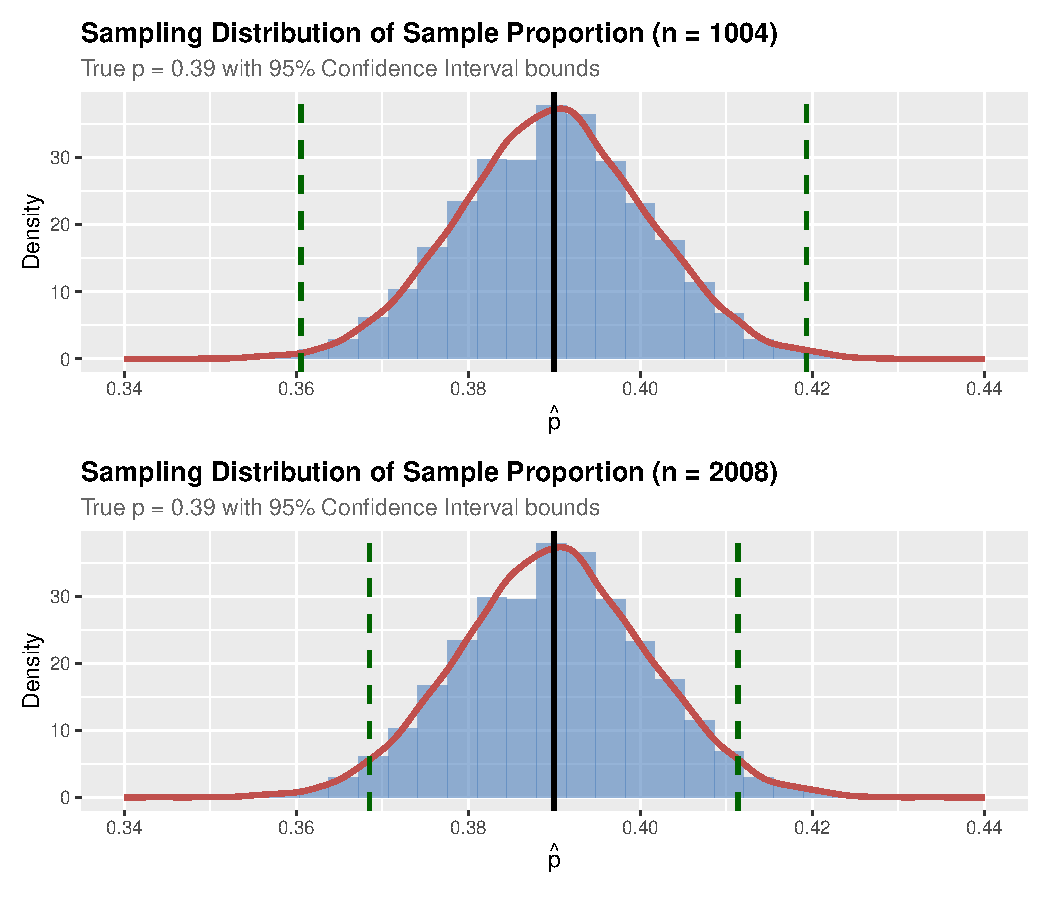
\includegraphics[width=\textwidth]{basic.sim.plots.pdf}
  \caption{Basic Sampling Distribution}
  \label{plot1}
  \end{center}
\end{figure}

\begin{figure}[H]
  \begin{center}
  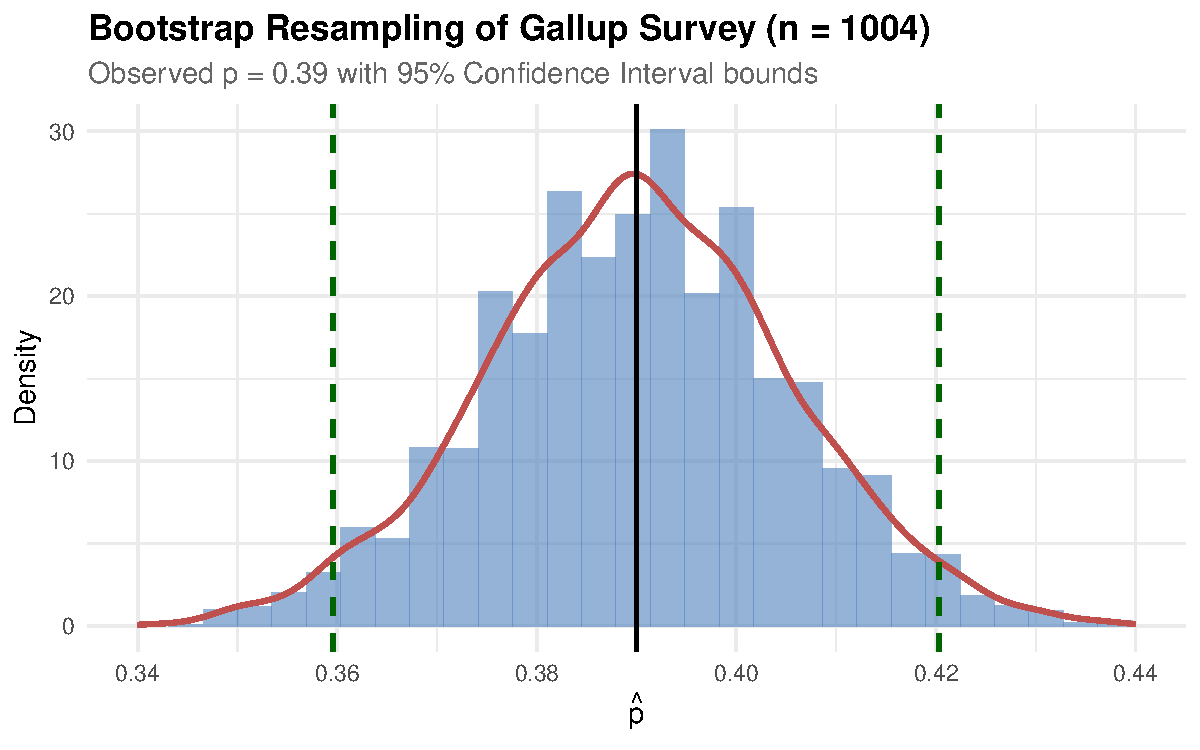
\includegraphics[width=\textwidth]{resample.plot.pdf}
  \caption{Resampling Plot}
  \label{plot2}
  \end{center}
\end{figure}

\begin{figure}[H]
  \begin{center}
  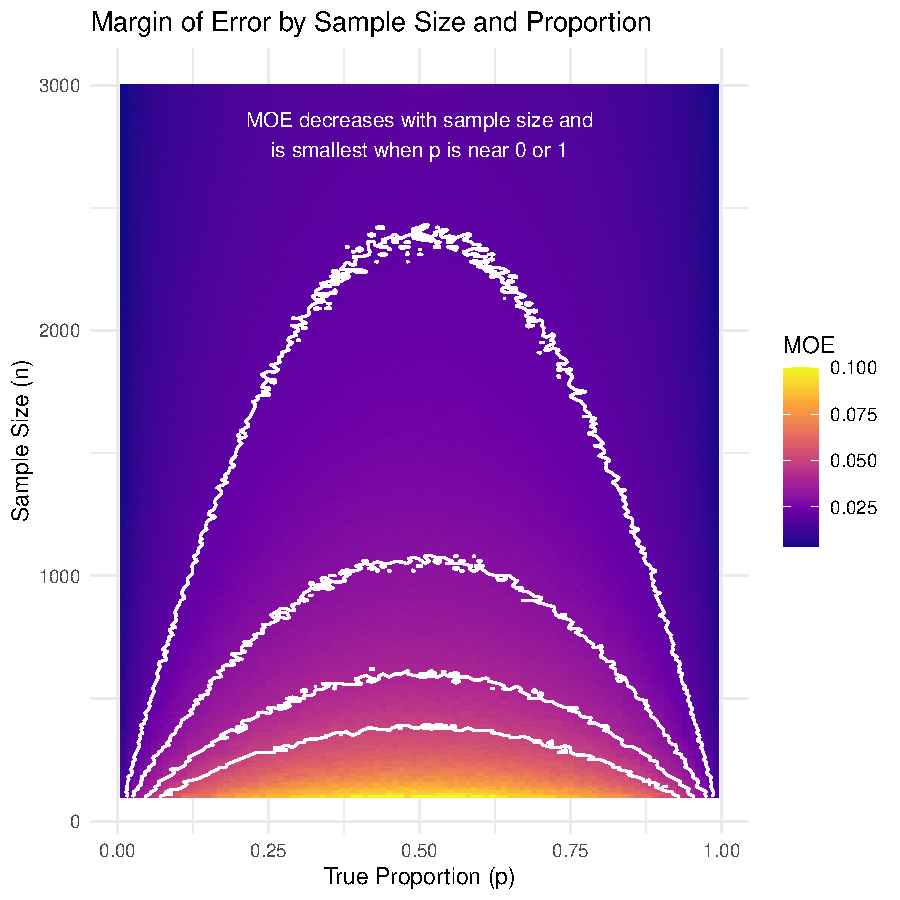
\includegraphics[width=\textwidth]{moe.heatmap.pdf}
  \caption{MOE Heat Map for simulation over $n$ and $p$}
  \label{plot3}
  \end{center}
\end{figure}

\begin{figure}[H]
  \begin{center}
  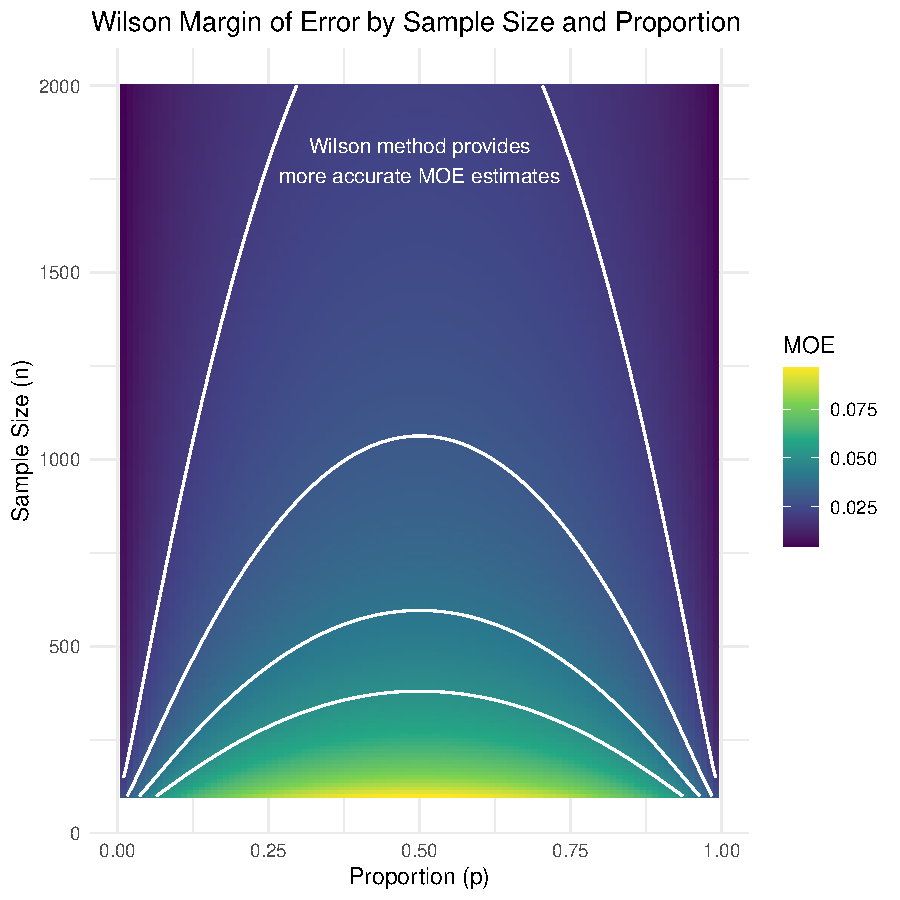
\includegraphics[width=\textwidth]{wilson.heatmap.pdf}
  \caption{Wilson Heat Map for simulation over $n$ and $p$}
  \label{plot4}
  \end{center}
\end{figure}

\end{document}
